% Generated by analyze_t1.js - requires \usepackage{pgfplots} and \pgfplotsset{compat=1.18}
\begin{figure}[t]
\centering
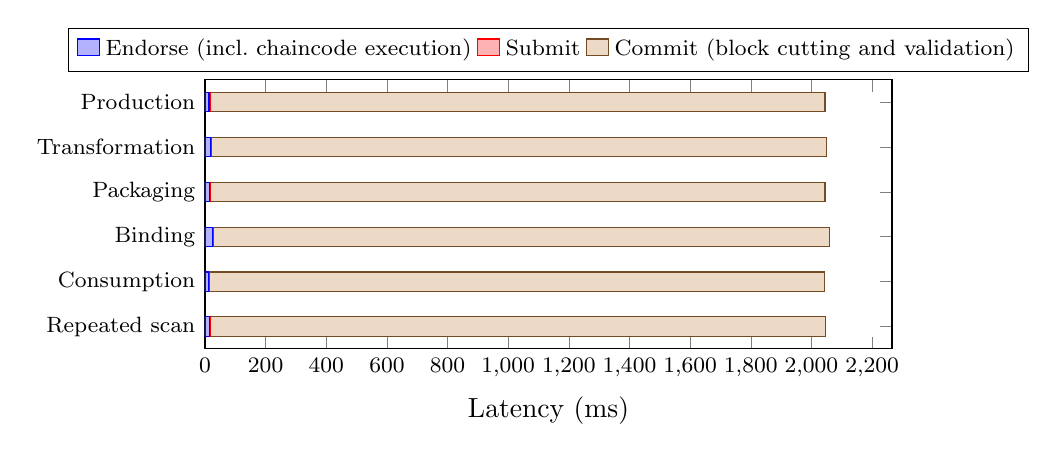
\begin{tikzpicture}
\begin{axis}[xbar stacked, width=0.85\linewidth, height=5cm, bar width=7pt,
  symbolic y coords={Production,Transformation,Packaging,Binding,Consumption,Repeated scan}, ytick=data, y dir=reverse, xmin=0,
  xlabel={Latency (ms)}, tick label style={font=\footnotesize},
  legend style={font=\footnotesize, at={(0.5,1.03)}, anchor=south, legend columns=3}]
\addplot coordinates {(13.2,Production) (17.9,Transformation) (14.1,Packaging) (25.5,Binding) (12.0,Consumption) (16.3,Repeated scan)};
\addplot coordinates {(3.3,Production) (2.9,Transformation) (2.7,Packaging) (2.8,Binding) (2.6,Consumption) (2.8,Repeated scan)};
\addplot coordinates {(2028.1,Production) (2029.6,Transformation) (2028.1,Packaging) (2031.4,Binding) (2028.5,Consumption) (2028.7,Repeated scan)};
\legend{Endorse (incl.\ chaincode execution), Submit, Commit (block cutting and validation)}
\end{axis}
\end{tikzpicture}

\vspace{2mm}
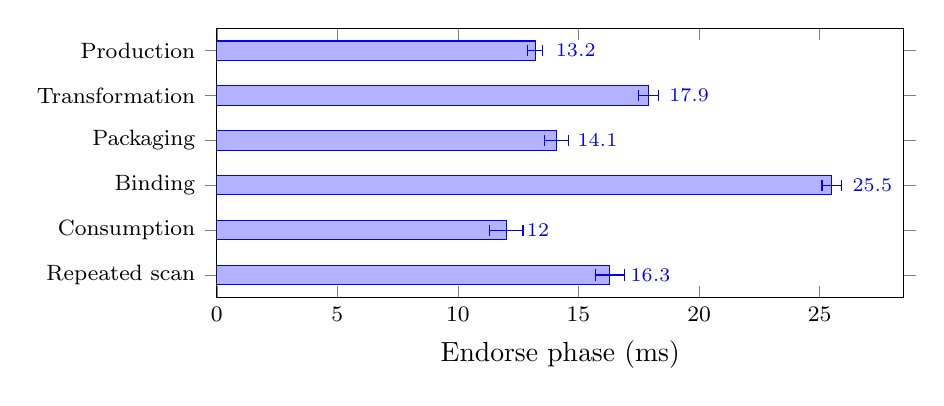
\begin{tikzpicture}
\begin{axis}[xbar, width=0.85\linewidth, height=5cm, bar width=7pt,
  symbolic y coords={Production,Transformation,Packaging,Binding,Consumption,Repeated scan}, ytick=data, y dir=reverse, xmin=0,
  xlabel={Endorse phase (ms)}, tick label style={font=\footnotesize},
  nodes near coords, nodes near coords style={font=\scriptsize, anchor=west, xshift=4pt},
  error bars/x dir=both, error bars/x explicit]
\addplot coordinates {(13.2,Production) +- (0.3,0) (17.9,Transformation) +- (0.4,0) (14.1,Packaging) +- (0.5,0) (25.5,Binding) +- (0.4,0) (12.0,Consumption) +- (0.7,0) (16.3,Repeated scan) +- (0.6,0)};
\end{axis}
\end{tikzpicture}
\caption{T1: decomposition of the latency of state-changing operations (top) and detail of the endorsement phase, which contains the chaincode execution (bottom; mean $\pm$ 95\% CI over runs).}
\label{fig:t1-decomposition}
\end{figure}
